%-------------------------------------------------------------
% FOLIACIÓN DE LA FRONTERA
%-------------------------------------------------------------

\subsection{Foliaci\'{o}n de la frontera}
\label{subsec:foliacionfrontera}

Consid\'{e}rese una regi\'{o}n $\Omega$ del espacio-tiempo foleada por hipersuperficies espacialoides $\Sigma_{t}$ cuya frontera son superficies (bidimensionales) cerradas $S_{t}$. $\partial \Omega$ es la uni\'{o}n de las hipersuperficies $\Sigma_{t_{1}}$, $\Sigma_{t_{2}}$ y $\mathcal{B}$ (con $\mathcal{B}$ la uni\'{o}n de todas las superficies $S_{t}$).

\begin{figure}[H]
\label{fig:OmegaandboundOmega}
\centering
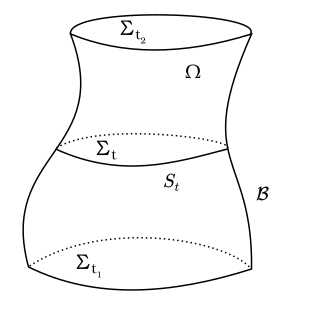
\includegraphics[width=0.3\textwidth]{Omega.png}
\caption{Regi\'{o}n $\Omega$, frontera $\partial \Omega$ y la foliaci\'{o}n.}
\end{figure}

Las superficies cerradas $S_{t}$ est\'{a}n descritas por las relaciones param\'{e}tricas $y^{a} (\theta^{w})$, donde $\theta^{w}$ son las coordenas en $S_{t}$. Se denota a $r_{a}$ como el vector normal a $S_{t}$ y se define un 4-vector asociado $r^{\alpha} = r^{a} e^{\alpha}_{a}$, que es ortogonal a $n_{\alpha}$ y satisface $r^{\alpha} r_{\alpha} = 1$.

Los vectores $e^{a}_{w} = \partial y^{a} / \partial \theta^{w}$ tangentes a $S_{t}$ expresados como 4-vectores se ven de la siguiente manera,
%
\begin{equation}
\label{eq:ealphaw}
e^{\alpha}_{w} = e^{\alpha}_{a} e^{a}_{w} = \frac{\partial x^{\alpha}}{\partial \theta^{w}}.
\end{equation}

La ecuaci\'{o}n \eqref{eq:ealphaw} ayuda a ver que las componentes de la m\'{e}trica $\sigma_{vw}$ inducida en $S_{t}$ est\'{a}n dadas por
%
\begin{equation}
\label{eq:metricSt}
\sigma_{vw} = h_{ab} e^{a}_{v} e^{b}_{w}
= (g_{\alpha \beta} e^{\alpha}_{a} e^{\beta}_{b}) e^{a}_{v} e^{b}_{w}
= g_{\alpha \beta} e^{\alpha}_{v} e^{\beta}_{w}.
\end{equation}
%
Y su inversa es denotada por $\sigma^{vw}$. Las relaciones de completez son $h^{ab} = r^{a} r^{b} + \sigma^{vw} e^{a}_{v} e^{b}_{w}$ y $g^{\alpha \beta} = -n^{\alpha} n^{\beta} + h^{ab} e^{\alpha}_{a} e^{\beta}_{b}$. Est\'{a} \'{u}ltima puede reescribirse como
%
\begin{equation}
\label{eq:complt}
g^{\alpha \beta} = -n^{\alpha} n^{\beta} + r^{\alpha} r^{\beta} + \sigma^{vw} e^{\alpha}_{v} e^{\beta}_{w}.
\end{equation}

La curvatura extr\'{i}nseca de $S_{t}$ encajada en $\Sigma_t$ est\'{a} definida por
%
\begin{equation}
\label{eq:extrinseccurvSt}
k_{vw} = e^{\alpha}_{v} e^{\beta}_{w} k_{\alpha \beta} = e^{\alpha}_{v} e^{\beta}_{w} \nabla_{\beta} r_{\alpha}.
\end{equation}
%
La traza de $k_{vw}$ no es m\'{a}s que $k = \sigma^{vw} k_{vw}$.

De manera similar a lo hecho en la secci\'{o}n \ref{subsec:3+1}, para relacionar las coordenadas $\theta^{w}$ de una superficie $S_{t}$ con las de otra superficie $S_{t}'$, se considera una congruencia de curvas $\beta$ en $\mathcal{B}$ que intersecten las superficies $S_{t}$ ortogonalmente, es decir, que vayan a lo largo de $n^{\alpha}$. Despu\'{e}s se pide que si la curva $\beta_{q}$ intersecta $S_{t}$ en $q$ con coordenada $\theta^{w}$, entonces la misma coordenada sea asignada en la intersecci\'{o}n de $\beta_{q}$ con $S_{t'}$ y as\'{i} sucesivamente.

La hipersuperficie $\mathcal{B}$ est\'{a} foleada por las superficies $S_{t}$. En principio, se puede ajustar a $\mathcal{B}$ un sistema coordenado arbitrario, sin embargo conviene escoger: $z^{f} = (t, \theta^{w})$. En \'{e}stas coordenadas $dx^{\alpha} = N n^{\alpha} dt + e^{\alpha}_{w} d \theta^{w}$, as\'{i} para desplazamientos dentro de $\mathcal{B}$ el elemento de l\'{i}nea es
%
\begin{align}
\label{eq:dsB}
ds_{\mathcal{B}} & = g_{\alpha \beta} (N n^{\alpha} dt + e^{\alpha}_{v} d \theta^{v}) (N n^{\beta} dt + e^{\beta}_{w} d \theta^{w}) \nonumber \\
& = - N^{2} dt^{2} + \sigma_{vw} d \theta^{v} d \theta^{w}.
\end{align}
%
Por otro lado, la m\'{e}trica inducida $\gamma_{fg}$ en $\mathcal{B}$ tiene componentes
%
\begin{equation}
\label{eq:indmetricB}
\gamma_{fg} = g_{\alpha \beta} \left( \frac{\partial x^{\alpha}}{\partial z^{f}} \right) \left( \frac{\partial x^{\beta}}{\partial z^{g}} \right) = g_{\alpha \beta} e^{\alpha}_{f} e^{\beta}_{g}
\end{equation}
%
y la inversa se denota por $\gamma^{fg}$. La relaci\'{o}n de completes toma la forma\footnote{Como $r^{\alpha}$ es ortogonal a $S_{t}$, tambi\'{e}n lo es a $\mathcal{B}$.}
%
\begin{equation}
\label{eq:Bcompltrelation}
g^{\alpha \beta} = r^{\alpha} r^{\beta} + \gamma^{fg} e^{\alpha}_{f} e^{\beta}_{g}.
\end{equation}

Ahora, de \eqref{eq:dsB} se sigue que
%
\begin{equation}
\gamma_{fg} dz^{f} dz^{g} =  - N^{2} dt^{2} + \sigma_{vw} d \theta^{v} d \theta^{w},
\end{equation}
%
por lo que implica $\sqrt{-\gamma} = N \sqrt{\sigma}$.

Por \'{u}ltimo,  la curvatura extr\'{i}nseca $\mathcal{K}_{fg}$ de $\mathcal{B}$ dentro del espacio-tiempo est\'{a} dada por
%
\begin{equation}
\mathcal{K}_{fg} = e^{\alpha}_{f} e^{\beta}_{g} \nabla_\beta r^{\alpha},
\end{equation}
%
y su traza por $\mathcal{K} = \gamma^{fg} \mathcal{K}_{fg}$.